\begin{figure*}[!t]
\begin{center}
\subfigure[Inconsistency over
  time]{\epsfig{file=dynamic/figures/TS_Peer3.eps,
    width=0.47\linewidth}}\hfill 
\subfigure[Inconsistency event duration
  distribution]{\epsfig{file=dynamic/figures/ED_Peer3.eps,
  width=0.47\linewidth}}\hfill 
\subfigure[Inconsistency across
  prefixes]{\epsfig{file=dynamic/figures/VP_Peer3.eps,
  width=0.47\linewidth}}\hfill 
%\begin{tabular}{ccc}
%\epsfysize=1.42in \epsffile{dynamic/figures/TS_Peer3.eps} & \epsfysize=1.42in
%\epsffile{dynamic/figures/ED_Peer3.eps} & \epsfysize=1.42in
%\epsffile{dynamic/figures/VP_Peer3.eps}\\ (a) Inconsistency over time & (b)
%Inconsistent event duration distribution & (c) Inconsistency across
%prefixes \\
%\end{tabular}

\caption{eBGP data analysis of a large tier-1 ISP peering with AT\&T.}
\label{fig:ebgp_result}
\end{center}
\end{figure*}

\begin{figure*}[!t]
\begin{center}
\begin{tabular}{cc}
\epsfysize=2.25in \epsffile{dynamic/figures/ED2.eps} & \epsfysize=2.25in
\epsffile{dynamic/figures/VP2.eps}\\ (a) Inconsistent event duration
distribution & (b) Inconsistency duration across prefixes\\
\end{tabular}
\centering
\caption{iBGP data analysis of several peers with AT\&T.}
\label{fig:ibgp_result}
\end{center}
\end{figure*}

%%%
%%% results.tex
%%%
\subsection{Measurement Results}
\label{sec:results}
%%%
%%% Intro
%%%

In this subsection, we apply the algorithms from
Sections~\ref{sec:problem} and~\ref{sec:algo} to the routing and
configuration data of AT\&T's commercial IP backbone.  We analyze both
the eBGP data from one of AT\&T's peers---a large tier-1 ISP---and the
iBGP data from the border routers in AT\&T's network (AS 7018) that
connect to peers over the period of May 1-8, 2004.  We verified that
AT\&T's import policies and peering sessions did not change during
this period, and that no resets occurred on the BGP sessions to
the route monitors.

\paragraph{Direct eBGP Feeds from One Peer} \label{subsec:ebgpResult}

We examine eBGP feeds from an AS with about half a dozen peering
points with AT\&T.  The data were obtained directly from the peer's
routers in the same PoPs as the eBGP sessions with AT\&T, and sometimes
from the same router that peers with AT\&T.  The route monitor
receiving these eBGP feeds is treated like a ``customer'' receiving a
complete routing table. To simulate the routes received by a peer like
AT\&T, we use community strings to distinguish customer routes from
peer routes.  Route advertisements that would not be advertised to a
peer are treated as withdrawals, since a BGP session with AT\&T would
not advertise these routes.
%\footnote{We cannot be entirely certain of the advertisements sent by
%the peer to AT\&T, because we do not know the peer's export policies;
%this could cause additional inconstencies.}
%Thus, our analysis provides a lower bound on the
%inconsistency from the peer to AT\&T's network.  
We identify two types of inconsistency in the eBGP feeds: missing
prefixes and differing AS path lengths.

Figure~\ref{fig:ebgp_result}(a) shows a time series of the total
number of inconsistent prefixes over the eight-day period of the
study. Fewer than five prefixes have inconsistent AS path lengths at
any given time, and most inconsistencies involve missing advertisements at
one or more peering points.
%We observe a
%sharp increase in the number of inconsistent prefixes on May 8th, but
Figure~\ref{fig:ebgp_result}(b) shows the complementary cumulative
distribution of the duration of the inconsistencies.  Most
inconsistencies last less than two minutes, suggesting that they are
caused by transient events such as routing protocol convergence.
Figure~\ref{fig:ebgp_result}(c) shows the overall duration of
inconsistencies for the prefixes advertised by this peer. The graph
shows that 70\% of the prefixes were {\em never\/} inconsistent, and
more than 97\% were inconsistent less than 0.23\% of the time.  Still,
a few inconsistencies due to missing advertisements persisted for
hours or even days.  A small number of prefixes were inconsistent for
the entire duration of the study, perhaps due to configuration
mistakes.
%
%0.0023283615906794      97.000764

%speculate:de-aggregation

\input{dynamic/iBGPresult}


\iffalse
Graph \#1: time series of inconsistency vs. time
\begin{itemize}
\item x-axis: time 
\item y-axis: percentage
\item curves: missing, length mismatch, and total
\end{itemize}


Graph \#2: fraction of time for inconsistencies (CCDF)
\begin{itemize}
\item x-axis: % of time
\item y-axis: % of prefixes inconsistent for time x or longer
\item curves: missing, length mismatch, and total
\item note: we may put y-axis on log scale to highlight the tail
\end{itemize}

Graph \#3: duration of inconsistencies (CDF)
\begin{itemize}
\item x-axis: duration of time
\item y-axis: % of events with duration x or less
\item curves: missing, length mismatch, and total
\end{itemize}
\fi
